\documentclass[aspectratio=169]{beamer}

\usepackage[utf8]{inputenc}
\usepackage[natbibapa]{apacite}
\usepackage{fancyhdr}
\renewcommand{\familydefault}{\sfdefault}

\title{Imposter Syndrome}
\author{Bianca Gibson}
\institute{Pycon AU 2016}
\date{}

\begin{document}

\frame{\titlepage}

\begin{frame}
  \begin{center}
    \Huge `the experience of fraudulent thoughts and feelings and the inability to attribute and internalize personal achievement'
    \\ \small \cite{hh15}
  \end{center}
\end{frame}

\begin{frame}
  \begin{center}
    \Huge Do you have it?
  \end{center}
\end{frame}

\begin{frame}
  \begin{center}
    \Huge How does it work?
  \end{center}
\end{frame}

\begin{frame}
  \begin{center}
    \Huge Consequences
  \end{center}
\end{frame}

\begin{frame}
  \begin{center}
    \Huge Dealing with it
  \end{center}
\end{frame}

\begin{frame}
  \begin{center}
    \Huge Are any of these true for you?
    \\ \small \cite{clance85}
  \end{center}
\end{frame}

\begin{frame}
  \begin{center}
    \Huge  I have often succeeded on a test or task even though I was afraid that I would not do well before I undertook the task
  \end{center}
\end{frame}

\begin{frame}
  \begin{center}
    \Huge  I can give the impression that I’m more competent than I really am
  \end{center}
\end{frame}

\begin{frame}
  \begin{center}
    \Huge  I avoid evaluations if possible and have a dread of others evaluating me
  \end{center}
\end{frame}

\begin{frame}
  \begin{center}
    \Huge  When  people  praise  me  for  something  I’ve  accomplished,  I’m  afraid  I  won’t  be able to live up to their expectations of me in the future
  \end{center}
\end{frame}

\begin{frame}
  \begin{center}
    \Huge  I sometimes think I obtained my present position or gained my present success because I happened to be in the right place at the right time or knew the right people
  \end{center}
\end{frame}

\begin{frame}
  \begin{center}
    \Huge  I’m  afraid  people  important  to  me  may  find  out  that  I’m  not  as  capable  as  they  think  I  am
  \end{center}
\end{frame}

\begin{frame}
  \begin{center}
    \Huge I tend to remember the incidents in which I have not done my best more than those times I have done my best
  \end{center}
\end{frame}

\begin{frame}
  \begin{center}
    \Huge  I rarely do a project or task as well as I’d like to do it
  \end{center}
\end{frame}

\begin{frame}
  \begin{center}
    \Huge  Sometimes I feel or believe that my success in my life or in my job has been the result of some kind of error
  \end{center}
\end{frame}

\begin{frame}
  \begin{center}
    \Huge    It’s  hard  for  me  to  accept  compliments  or  praise  about  my  intelligence  or  accomplishments
  \end{center}
\end{frame}

\begin{frame}
  \begin{center}
    \Huge At times, I feel my success has been due to some kind of luck
  \end{center}
\end{frame}

\begin{frame}
  \begin{center}
    \Huge   I’m  disappointed  at  times  in  my  present  accomplishments  and  think  I should have accomplished much more
\end{center}
\end{frame}

\begin{frame}
  \begin{center}
    \Huge   Sometimes I’m afraid others will discover how much knowledge or ability I really lack
  \end{center}
\end{frame}

\begin{frame}
  \begin{center}
    \Huge     I’m  often  afraid  that  I  may  fail  at  a  new  assignment  or  undertaking  even  though  I  generally  do  well  at  what  I
  attempt
\end{center}
\end{frame}

\begin{frame}
  \begin{center}
    \Huge   When  I’ve  succeeded  at  something  and  received  recognition  for  my  accomplishments,  I  have  doubts  that I can keep repeating that success
\end{center}
\end{frame}

\begin{frame}
  \begin{center}
    \Huge     If  I  receive  a  great  deal  of  praise  and  recognition  for  something  I’ve  accomplished,  I  tend  to  discount  the  importance
  of  what  I’ve  done
\end{center}
\end{frame}

\begin{frame}
  \begin{center}
    \Huge     I often compare my ability to those around me and think they may be more intelligent than I am
  \end{center}
\end{frame}

\begin{frame}
  \begin{center}
    \Huge      I often worry about not succeeding with a project or examination, even though others around me have considerable
confidence that I will do well
\end{center}
\end{frame}

\begin{frame}
  \begin{center}
    \Huge       If  I’m  going  to  receive  a  promotion  or  gain  recognition  of  some  kind,  I  hesitate  to  tell  others  until  it  is  an
  accomplished fact
\end{center}
\end{frame}

\begin{frame}
  \begin{center}
    \Huge  I  feel  bad  and  discouraged  if  I’m  not  `the  best'  or  at  least  `very  special'  in  situations  that  involve  achievement
\end{center}
\end{frame}

\begin{frame}
  \begin{center}
    \Huge Who has it?
    \\ \small \cite{clanceimes78}
    \\ \small \cite{attr98}
    \\ \small \cite{colour}
    % initially discovered in high achieving women studying and in academia
    % later found in to be in other populations too
    % Maybe higher in women, research goes both ways
    % Maybe higher in some ethnic groups, studied in African Americans
  \end{center}
\end{frame}

\begin{frame}
  \begin{center}
    \Huge Minorities
    \\ \small \cite{apa13}
  \end{center}
\end{frame}

\begin{frame}
  \begin{center}
    \Huge New endeavour
    \\ \small \cite{apa13}
    % me with the greens - Apsara & Asher suggesting I go for council
  \end{center}
\end{frame}

\begin{frame}
  \begin{center}
    \Huge What are the characteristics?
  \end{center}
\end{frame}

\begin{frame}
  \begin{center}
    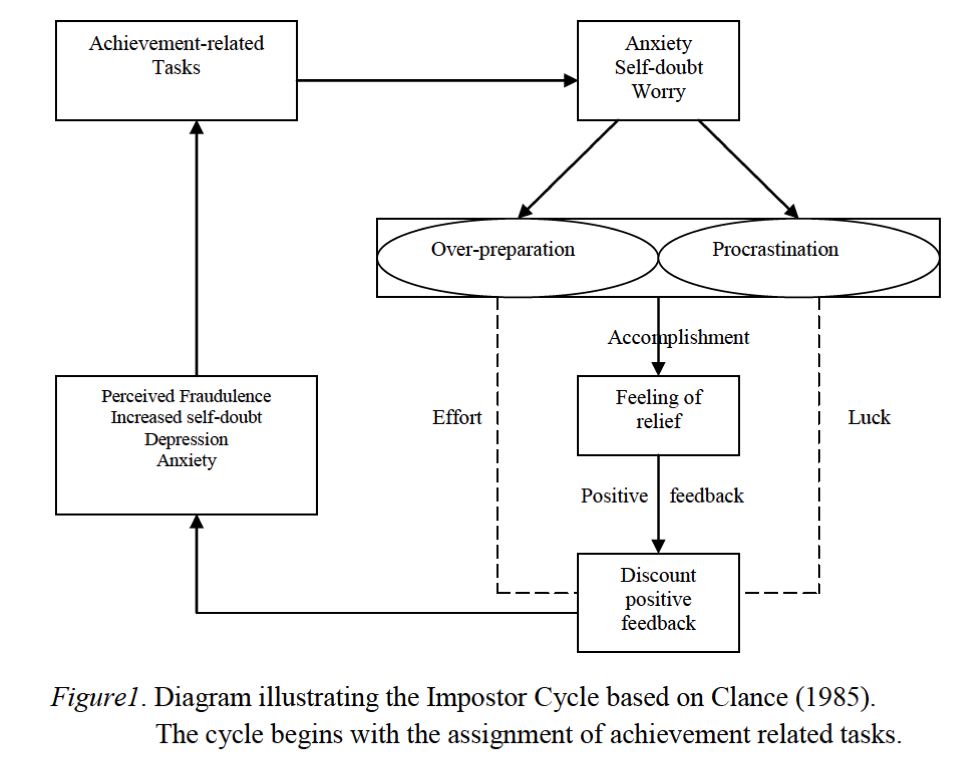
\includegraphics[scale=.5]{./assets/clance-impostor-cycle.png}
    \\ \small \cite{sakulku11}
  \end{center}
\end{frame}

\begin{frame}
  \begin{center}
    \Huge How does it work?
    % attribute successes to outside factors - luck, colleagues
    % attribute failures to themselves
    % found to be far more common in women than men
    % women viewing ourselves as phony is consistent with societal view that we aren't competent
    % worse for African American women
    % easier to not internalize success than go against the views of society!
    % often seem to perservere despite that, some desire to prove society and themselves wrong
    % often believe that intelligence is fixed rather than malleable
    % motivated by performance goals, try to prove intelligence
    % when fail - react 'helpless' way, blame selves, withdraw from task, anxiety, shame
    % overriding concern with others' impressions, idealised self image
    % self worth unusually dependent on others - external validation goes away, fall apart
    \\ \small \cite{hh15}
    \\ \small \cite{langford93}
    \\ \small \cite{colour}
  \end{center}
\end{frame}

\begin{frame}
  \begin{center}
    \Huge Success does not fix it
    \\ \small \cite{clanceimes78}
    \\ \small \cite{sakulku11}
    % because they dismiss the success
    % disregard if there is any gap between their expectations and performance
    % repetitions of success show dif between actual and ideal standards, make it worse
    % deny our competence, discount praise
  \end{center}
\end{frame}

\begin{frame}
  \begin{center}
    \Huge Desire to be the best
    % will be the biggest fish in a small pond (school)
    % then go to uni - lots of bright people, not the best anymore
    % conclude that they are stupid because they aren't the best anymore
    \\ \small \cite{sakulku11}
  \end{center}
\end{frame}

\begin{frame}
  \begin{center}
    \Huge Fear and guilt about success
    \\ \small \cite{sakulku11}
  \end{center}
\end{frame}

\begin{frame}
  \begin{center}
    \Huge Defendence
    \\ \small \cite{langford93}
    % mistrusting others
  \end{center}
\end{frame}

\begin{frame}
  \begin{center}
    \Huge Low affiliation
    \\ \small \cite{langford93}
    % in women. enjoyable involvement with other people
  \end{center}
\end{frame}

\begin{frame}
  \begin{center}
    \Huge Low play
    \\ \small \cite{langford93}
    % don't do things for fun
  \end{center}
\end{frame}

\begin{frame}
  \begin{center}
    \Huge Impulsivity
    \\ \small \cite{langford93}
    % low in women, high in men
  \end{center}
\end{frame}

\begin{frame}
  \begin{center}
    \Huge Need for change
    \\ \small \cite{langford93}
    % low in women, high in men
  \end{center}
\end{frame}

\begin{frame}
  \begin{center}
    \Huge Low need for order
    \\ \small \cite{langford93}
    % in men
  \end{center}
\end{frame}

\begin{frame}
  \begin{center}
    \Huge What childhood circumstances create it?
    \\ \small \cite{sakulku11}
    \\ \small \cite{langford93}
    % Generally either has a sibling or close relative that was the designated 'intelligent' family member
    % the woman is then told that she is the 'sensitive' or socially adept one, not the smart one
    % or, told that they are superior in every way and success will come easily
    % Then they can't cope with when it doesn't
    % Family valueing success with little effort
    % descrepency between feedback and actual success
    % lack of positive reinforcement - ``nothing you do is ever good enough''
    % IP higher when family cohesion and expressiveness are low, family conflict and control high. Accounted for 12% of variation
    % if not supported or approved may feel achievements are dismissed, unimpressive, unimportant.
    % shame, humiliation and inauthenticity common with lack of +ve reinforcement
    % IP highly correlated with need to please others in family
    % try to live up to idealised image to win approval
  \end{center}
\end{frame}

\begin{frame}
  \begin{center}
    \Huge Personality traits
    % "common among individuals with particular personality traits (e.g. neuroticism, achievement-orientation), have perfectionist expectations over work"
    % inverse with conscientiousness
    \\ \small \cite{hh15}
    \\ \small \cite{sakulku11}
  \end{center}
\end{frame}

\begin{frame}
  \begin{center}
    \Huge Work circumstances that contribute
    % "and who work in highly competitive, stressful occupations similar to that of the academic environment"
    % what about peer review?
    % higher in untenured faculty - probably maps to staff on fixed term contracts
    % not studied in tech, but higher in systems librarians than other librarians
    % high tech knowledge requirements, constant technical change, feel out of date
    \\ \small \cite{hh15}
    \\ \small \cite{clark14}
  \end{center}
\end{frame}

\begin{frame}
  \begin{center}
    \Huge Racial issues
    \\ \small \cite{colour}
    % studied in African Americans
    % people's presumed incompetence in African American women
    % vital for them to establish self worth and self reliance - others assessment will be unfairly negative
    % Group counselling with other African American women is very effective
    % more comfortable with people like them, see the ridicilousness of others IP
    % similar situation -> share strategies
  \end{center}
\end{frame}

\begin{frame}
  \begin{center}
    \Huge Self presentation
    \\ \small \cite{sakulku11}
    % Do not want to appear imperfect, but actually openly disclose their imperfection.
    % Is it an interpersonal strategy rather than self evalution?
    % could be to avoid negative interpersonal implications of future failures
    % only express lower performance expectations when they know others see it
    % correlated with other favourale impression management strategies
    % makes *lots* of sense for women in tech, since being seen as competetent makes you less likeable
  \end{center}
\end{frame}

\begin{frame}
  \begin{center}
    \Huge Behaviours that preserve it
  \end{center}
\end{frame}

\begin{frame}
  \begin{center}
    \Huge Intellectual Inauthenticity
    \\ \small \cite{clanceimes78}
    % chose not to reveal ideas or opinions
    % tell people what they want to hear
    % intellectual flattery - writing according to their teachers' biases
    % or for a developer - implementing it how the more senior developers or tech lead would want, not what you think is best
    % remaining silent in face of opposing view points
    % prevents them from finding out what people would think of their authentic views
    % maintains imposter syndrome
  \end{center}
\end{frame}

\begin{frame}
  \begin{center}
    \Huge Charm
    \\ \small \cite{clanceimes78}
    %"Typically, she believes, "I am stupid," but at anther
    %level  she  believes  she  is  brilliant,  creative,  and  special  if  only  the  right  person  would  discover
    %her genius and thereby help her believe in her intellect. "
    % aim to be liked as well as recognised intellectually
    % finds a candidate she respects, then tries to impress to gain approval
    % studies them, figures out how to impress them, sets about winning them over
    % may pick up ttheir hobbies
    % listens with understanding and concern
    % usually gains approval, but doesn't work
    % will never believe the praise because it's based on liking her
    % if she was really that bright, would she need the outside approval?
  \end{center}
\end{frame}

\begin{frame}
  \begin{center}
    \Huge Avoiding displays of confidence
    \\ \small \cite{clanceimes78}
    % find a recent quote for success going against likeability for women
    % Many women have a motive to avoid success, a well justified fear of rejection or less feminine if they do
    % look at all the crap Julia Gillard put up with - quote from her speech
    % pattern of tight roping
    % denying their success allows them to live out achievement orientation while allaying some fears about being a successful women
  \end{center}
\end{frame}

\begin{frame}
  \begin{center}
    \Huge What are the consequences?
  \end{center}
\end{frame}

\begin{frame}
  \begin{center}
    \Huge Poor mental health
    \\ \small \cite{sakulku11}
  \end{center}
\end{frame}

\begin{frame}
  \begin{center}
    \Huge Bouts of depression and anxiety
    \\ \small \cite{hh15}
  \end{center}
\end{frame}

\begin{frame}
  \begin{center}
    \Huge Emotional exhaustion
    \\ \small \cite{hh15}
    % stress part of burnout - fatigue, depression, emotional and cognitive distancing -> low work satisfaction and performance
  \end{center}
\end{frame}


\begin{frame}
  \begin{center}
    \Huge Psychological distress
    \\ \small \cite{hh15}
  \end{center}
\end{frame}

\begin{frame}
  \begin{center}
    \Huge Low self confidence
    \\ \small \cite{hh15}
  \end{center}
\end{frame}

\begin{frame}
  \begin{center}
    \Huge Adversely related to job well-being, satisfaction and performance
    \\ \small \cite{hh15}
  \end{center}
\end{frame}

\begin{frame}
  \begin{center}
    \Huge Low self-efficacy
    \\ \small \cite{feedback}
    % attribute initial success to ability -> higher self efficacy
    % higher self efficacy related to higher performance
    % leads to higher self efficacy
    % performance analysis in early life super important - provides anchor, influencing later attribution
  \end{center}
\end{frame}

\begin{frame}
  \begin{center}
    \Huge Ways to cope
  \end{center}
\end{frame}

\begin{frame}
  \begin{center}
    \Huge Mentoring
    \\ \small \cite{hh15}
    % They can normalise the feelings
    % emotional support
    % instrumental support (tangible help with specific problems)
    % challenge to accept praise
    % even helpful if they don't discuss IP
    % mentors can be the target of unfair comparisons - 67% don't directly discuss with mentor
  \end{center}
\end{frame}

\begin{frame}
  \begin{center}
    \Huge Positive reinforcement
    \\ \small \cite{hh15}
    % greens appreciation letters (include photo)
  \end{center}
\end{frame}

\begin{frame}
  \begin{center}
    \Huge Identify feelings
    \\ \small \cite{caltech}
    % awareness is first step to change
  \end{center}
\end{frame}

\begin{frame}
  \begin{center}
    \Huge Reality check
    \\ \small \cite{caltech}
    % question the thoughts
  \end{center}
\end{frame}

\begin{frame}
  \begin{center}
    \Huge Differentiate between feelings and reality
    \\ \small \cite{caltech}
  \end{center}
\end{frame}

\begin{frame}
  \begin{center}
    \Huge Humor
    \\ \small \cite{hh15}
  \end{center}
\end{frame}

\begin{frame}
  \begin{center}
    \Huge Distracting thoughts or activities
    \\ \small \cite{hh15}
  \end{center}
\end{frame}

\begin{frame}
  \begin{center}
    \Huge Social support
    \\ \small \cite{caltech}
    % discuss feelings, get perspective
  \end{center}
\end{frame}

\begin{frame}
  \begin{center}
    \Huge Reduce dependency
    \\ \small \cite{langford93}
    % on external validation for self esteem
    % internalise self worth
  \end{center}
\end{frame}

\begin{frame}
  \begin{center}
    \Huge What to do?
    % steps to help yourself and others who experience IP
  \end{center}
\end{frame}

\begin{frame}
  \begin{center}
    \Huge Talk about it
    % discuss it in your workplace
    % like the group therapy sessions
  \end{center}
\end{frame}

\begin{frame}
  \begin{center}
    \Huge Be aware when people show it
    % yourself and others
    % I had such bad IP I thought 'they have IP, but I'm right!'
  \end{center}
\end{frame}

\begin{frame}
  \begin{center}
    \Huge Challenge people to accept positive feedback
  \end{center}
\end{frame}

\begin{frame}
  \begin{center}
    \Huge Get perspective
    % from people that will evaluate you fairly
    % don't charm them
  \end{center}
\end{frame}

\begin{frame}
  \begin{center}
    \Huge Questions?
  \end{center}
\end{frame}

\begin{frame}
 \bibliographystyle{apacite}

  \bibliography{./slides}
\end{frame}

\end{document}
